\documentclass[
12pt, % The default document font size, options: 10pt, 11pt, 12pt
oneside, % Two side (alternating margins) for binding by default, uncomment to switch to one side
english, % ngerman for German
onehalfspacing, % Single line spacing, alternatives: singlespacing, onehalfspacing or doublespacing
%draft, % Uncomment to enable draft mode (no pictures, no links, overfull hboxes indicated)
nolistspacing, % If the document is onehalfspacing or doublespacing, uncomment this to set spacing in lists to single
%liststotoc, % Uncomment to add the list of figures/tables/etc to the table of contents
%toctotoc, % Uncomment to add the main table of contents to the table of contents
%parskip, % Uncomment to add space between paragraphs
%nohyperref, % Uncomment to not load the hyperref package
headsepline, % Uncomment to get a line under the header
%chapterinoneline, % Uncomment to place the chapter title next to the number on one line
%consistentlayout, % Uncomment to change the layout of the declaration, abstract and acknowledgements pages to match the default layout
]{MastersDoctoralThesis} % The class file specifying the document structure
% Hairong Bau (2024, 2025, 2026)


\usepackage[utf8]{inputenc} % Required for inputting international characters
\usepackage[T1]{fontenc} % Output font encoding for international characters

\usepackage{mathpazo} % Use the Palatino font by default
\usepackage{pgfgantt}
%\usepackage{marginnote}

% Include Packages
%\usepackage[a4paper,inner=3.5cm,outer=2.5cm,top=2.5cm,bottom=2.5cm]{geometry}  % Set page margins
%\usepackage{fullpage}
\usepackage{float}                  % Allows 'Here and Only Here' [H] for Floats
\usepackage{url}                    % \url{} command
%\usepackage{charter}                  % Set font to Times
\usepackage{graphicx}               % \includegraphics
%\usepackage{subfigure}              % Allow subfigures
\usepackage{amsmath}
\usepackage{amssymb}
\usepackage{amsthm}

\usepackage{svg}
\usepackage{rotating}
\usepackage{mathtools}

\usepackage{enumitem}
\usepackage{booktabs}

\usepackage{pifont}
\usepackage{pdfpages}

\usepackage{algorithm}
\usepackage{algpseudocode}

\setlist[enumerate]{noitemsep, nolistsep}
\setlist[itemize]{noitemsep, nolistsep}
\setlist[description]{noitemsep, nolistsep}

\usepackage{geometry}
\usepackage{parskip}
%\usepackage{fancyhdr}
\usepackage[all]{nowidow}
\setnoclub[2]
\setnowidow[2]

% Referencing
% Provides \Vref and \vref to indicate where a reference is.
\usepackage{varioref} 
% Hyperlinks references
\usepackage[bookmarks=true,bookmarksopen=true]{hyperref} 
% Provides \Cref, \cref, \Vref, \vref to include the type of reference: fig/eqn/tbl
\usepackage{cleveref} 
% Setup Hyperref
\hypersetup{
  colorlinks   = true,              %Colours links instead of ugly boxes
  urlcolor     = blue,              %Colour for external hyperlinks
  linkcolor    = blue,              %Colour of internal links
  citecolor    = blue                %Colour of citations
}
% Names for Clever Ref
\crefname{table}{table}{tables}
\Crefname{table}{Table}{Tables}
\crefname{figure}{figure}{figures}
\Crefname{figure}{Figure}{Figures}
\crefname{equation}{equation}{equations}
\Crefname{equation}{Equation}{Equations}

% Wits Citation Style
\usepackage{natbib} \input{natbib-add}
\bibliographystyle{apalike}
\bibpunct{[}{]}{;}{a}{}{}  % to get correct punctuation for bibliography
\setlength{\skip\footins}{1.5cm}

%----------------------------------------------------------------------------------------
%	MARGIN SETTINGS
%----------------------------------------------------------------------------------------
\geometry{
	paper=a4paper, % Change to letterpaper for US letter
	inner=2.5cm, % Inner margin
	outer=3.8cm, % Outer margin
	bindingoffset=.5cm, % Binding offset
	top=1.5cm, % Top margin
	bottom=1.5cm, % Bottom margin
	%showframe, % Uncomment to show how the type block is set on the page
}

 
\newcommand{\citets}[1]{\citeauthor{#1}'s \citeyearpar{#1}}
\renewcommand\bibname{References}  

%----------------------------------------------------------------------------------------
%	THESIS INFORMATION
%----------------------------------------------------------------------------------------
\thesistitle{Mass Spectrometry Imaging and Peak Picking} % Your thesis title, this is used in the title and abstract, print it elsewhere with \ttitle
\author{Zayd \textsc{Suliman}} % Your name, this is used in the title page and abstract, print it elsewhere with \authorname



\begin{document}

\frontmatter % Use roman page numbering style (i, ii, iii, iv...) for the pre-content pages

\pagestyle{plain} % Default to the plain heading style until the thesis style is called for the body content

%----------------------------------------------------------------------------------------
%	TITLE PAGE
%----------------------------------------------------------------------------------------
\begin{titlepage}
\linespread{1}
\begin{center}
  \vspace*{.06\textheight}
  
\includegraphics[width=0.18\textwidth]{images/witslogonew.png}~\\[20pt]
  \Large \textsc{Literature Review}\\[12pt]
  {\huge \bf \ttitle}\\[20pt]  
  {\Large \bf \authorname}\\
  {\Large 2653934}\\[20pt]
  \large School of Computer Science and Applied Mathematics\\
  \large Faculty of Science\\
  \large University of the Witwatersrand\\[20pt]
  Supervisor: \\ Hairong Bau and Richard Klein
  \vfill
  \today
  %\vfill
  %
\includegraphics[width=1.5cm]{images/wits}
  %\vspace{10pt}\\
\end{center}
\end{titlepage} 

%----------------------------------------------------------------------------------------
%	DECLARATION PAGE
%----------------------------------------------------------------------------------------

% \begin{declaration}
% \addchaptertocentry{\authorshipname} % Add the declaration to the table of contents


% \end{declaration}

%----------------------------------------------------------------------------------------
%	ABSTRACT PAGE
%----------------------------------------------------------------------------------------
% --- Uncomment when an abstract is to be included
%%
\begin{abstract}
\addchaptertocentry{\abstractname} % Add the abstract to the table of contents 

Mass Spectrometry Imaging (MSI) is a revolutionary molecular microscopy technique that maps the spatial distribution of biomolecules within intact tissues, offering profound insights for precision medicine. However, the immense high-dimensional data generated by MSI is currently bottlenecked by heuristic preprocessing pipelines, specifically manual "peak picking." These classical algorithms introduce severe subjective bias, frequently discarding critical low-abundance disease biomarkers and distorting non-linear spectral manifolds. To overcome this limitation, this research proposes "Spatial-msiPL," a Spatially-Aware Variational Autoencoder designed for autonomous peak learning. By mathematically integrating physical neighborhood covariance into the encoding process via contextual input vectors and an explicit spatial coherence penalty, this lightweight 1D model aims to isolate true biomolecular signals from stochastic matrix noise. The proposed methodology will benchmark the extracted spatial ion images against expert-annotated structural segmentation masks using the mean Spatial F1-score (mSCF1). If successful, this framework will contribute a computationally efficient, spatially-aware alternative to heavy 3D convolutional networks, eliminating human bias and improving the clinical scalability of spatial omics analysis.
\end{abstract}

%----------------------------------------------------------------------------------------
%	ACKNOWLEDGEMENTS
%----------------------------------------------------------------------------------------
% \begin{acknowledgements}
% \addchaptertocentry{\acknowledgementname} % Add the acknowledgements to the table of contents
% The acknowledgments and the people to thank go here \ldots
% \end{acknowledgements}


%----------------------------------------------------------------------------------------
%	LIST OF CONTENTS/FIGURES/TABLES PAGES
%----------------------------------------------------------------------------------------
\tableofcontents % Prints the main table of contents

% --- Comment the following lines if ou don't have any figures/tables. 

% \listoffigures % Prints the list of figures

% \listoftables % Prints the list of tables

%\pagestyle{fancy}
%\fancyhf{}
%\fancyhead[LE,RO]{}
%\fancyhead[RE,LO]{\thepage}
%\renewcommand{\sectionmark}[1]{\chead{{\thesection \, #1}}}
%\fancyhead[CE,CO]{\thesection}
%\fancyfoot[CE,CO]{\leftmark}
%\fancyfoot[LE,RO]{\thepage}
%\renewcommand{\headrulewidth}{0.4pt}

%----------------------------------------------------------------------------------------
%	CONTENT - CHAPTERS
%----------------------------------------------------------------------------------------
\mainmatter % Begin numeric (1,2,3...) page numbering
\pagestyle{thesis} % Return the page headers back to the "thesis" style

% Include the chapters of the thesis as separate files from the Chapters folder
% Uncomment the lines as you write the chapters
%\include{Chapters/Introduction}
%\include{Chapters/Background} 
%\include{Chapters/Model}
%\include{Chapters/Method}
%\include{Chapters/ExperimentalSetup}
%\include{Chapters/ResultsDiscussion} 
%\include{Chapters/Conclusion}


\chapter{Introduction}
% --- Organize the contents in proper sections/subsections where necessary ---
% --- General problem area introduction to establish the main reseach field ---
% --- Motivation to show the research problem is important ---

The characterization of biological tissues has historically relied on classical histological staining and light microscopy, requiring anatomical pathologists to diagnose diseases based on structural and morphological cellular alterations. However, the paradigm of modern precision medicine necessitates a significantly deeper understanding of the molecular pathogenesis underlying these morphological changes. To bridge the gap between traditional histology and high-throughput molecular profiling, Mass Spectrometry Imaging (MSI), particularly Matrix-Assisted Laser Desorption/Ionization (MALDI), has emerged as a revolutionary molecular microscopy technique over the past three decades.~\citep{schwamborn2010molecular} By mapping the spatial distribution of thousands of distinct biomolecules ranging from small metabolites, lipids, and exogenous drugs to large intact proteins directly within an intact tissue section, MSI provides a label-free, highly multiplexed view of the cellular microenvironment.~\citep{ye2013msi}

The ability to simultaneously capture spatial relationships and complex spectral data without prior knowledge of the target molecules has propelled MSI to the forefront of contemporary biomedical research, facilitating advancements in biomarker discovery, pharmaceutical drug mapping, and clinical diagnostics~\citep{abdelmoula2021peak}. In complex localized pathologies such as glioblastoma, colorectal carcinoma, and infectious diseases, MSI enables the direct visualization of tumor heterogeneity, xenobiotic toxins, and localized immune responses that are otherwise entirely invisible to standard hematoxylin and eosin (H\&E) staining. Despite these profound advantages and the rapid maturation of the hardware, the clinical translation of MSI into routine diagnostic pipelines is heavily impeded by massive computational bottlenecks. A single high-resolution MSI experiment can generate three-dimensional data hypercubes ranging from tens of gigabytes to several terabytes per tissue slice~\citep{korber2025mass}. Each individual pixel within this spatial grid contains a high-dimensional mass spectrum, often consisting of tens to hundreds of thousands of discrete mass-to-charge ($m/z$) bins~\citep{abdelmoula2021peak}. Extracting biologically meaningful, statistically robust signals from this immense, noisy, and highly sparse data structure represents one of the most significant challenges in modern computational biology and medical image analysis~\citep{zhang2025msi_infectious}.

\section{Problem Statement}

Ideally, the computational analysis of clinical Mass Spectrometry Imaging datasets would be entirely automated, preserving the full spectrum of molecular information while seamlessly translating high-dimensional raw physical data into robust, clinically actionable diagnostic signatures. In such an ideal computational environment, machine learning models would accurately capture the highly non-linear relationships between thousands of interacting metabolites and proteins without requiring human bias or manual parameter intervention. This idealized pipeline would enable the immediate, unhindered identification of rare, low-abundance molecular biomarkers that are critical for the early detection and subtyping of complex diseases.

The reality of current MSI analysis, however, stands in stark contrast to this ideal. The conventional computational processing of MSI data is fundamentally limited by highly heuristic, multistep preprocessing pipelines that are required to compress the massive data hypercubes before any statistical analysis can occur. The most critical, computationally expensive, and subjective of these steps is "peak picking". Classical peak picking algorithms, such as those relying on sparse frame multipliers, continuous wavelet transforms, local maxima detection, or strict signal-to-noise ratio (SNR) thresholding, require extensive empirical parameter tuning~\citep{lieb2020sparse}.This subjectivity introduces a severe analytical bottleneck into the diagnostic pipeline: arbitrary thresholds inevitably discard low-abundance molecular signals, permanently masking crucial biological phenomena, while simultaneously retaining highly structured chemical noise derived from the matrix application process. Furthermore, traditional peak picking fundamentally destroys the underlying non-linear spectral manifold of the data, forcing all downstream machine learning classifiers and clustering algorithms to operate on a highly biased, artificially truncated, and linear representation of the tissue microenvironment. \citep{abdelmoula2021peak}

To propose an improvement to this reality and transition the field toward the ideal analytical environment, it is proposed that unsupervised deep learning models be deployed directly on raw, un-preprocessed MSI data arrays. Artificial neural networks, specifically deep generative models such as Variational Autoencoders (VAEs) and contrastive representation learning networks, possess the mathematical capacity to learn the generative physical processes and spatial correlations of molecular ions without requiring heuristic thresholding or prior baseline correction~\citep{abdelmoula2021peak}. By reconceptualizing peak detection not as an arbitrary signal-filtering task, but as an advanced manifold learning and spatial representation problem (often termed "peak learning) deep neural networks can autonomously discover biologically relevant $m/z$ features while retaining the complex, non-linear structural relationships inherent in the raw mass spectrometry data. Developing, evaluating, and optimizing these advanced deep learning frameworks, particularly for highly diverse and noisy datasets sourced from local clinical hospital environments, forms the core research imperative of this study. \citep{guo2024deepion}

%\chapter{Background} --- optional
% \chapter{Related Work}
\chapter{Background and Related Work}
%\section{Background} --- optional
\section{Background: Foundations of MSI}

Mass Spectrometry Imaging represents a profound technological intersection between advanced analytical chemistry, physics, and spatial biology. The technology functions by systematically directing a highly focused ionization source across a meticulously defined two-dimensional grid superimposed on a thin biological tissue section. In the MALDI MSI workflow, the tissue is coated with an energy-absorbing organic matrix. A pulsed laser is fired at discrete coordinates, sublimating the matrix and inducing localized desorption and ionization of the endogenous tissue molecules. An analyzer then separates the ions based entirely on their mass-to-charge ratio ($m/z$).\citep{caprioli1997maldi, korber2025mass}

The resulting computational output is an exceptionally high-dimensional data hypercube. For a tissue section imaged at a specific spatial resolution yielding $N \times M$ spatial pixels, each individual pixel contains a complete mass spectrum. This structural complexity creates a profound "curse of dimensionality," where the sheer volume of data rapidly exceeds the capacities of standard analytical workstations. \citep{abdelmoula2021peak, aspect2026msi_intro}

Due to the immense size, sparsity, and inherent noise of the raw spectral hypercube, classical workflows dictate the application of a heuristic-driven preprocessing pipeline (baseline subtraction, spectral smoothing, intensity normalization, and peak picking) prior to any downstream analysis. Peak picking, the most critical dimensionality reduction step, searches for local maxima that satisfy rigidly defined geometric criteria or SNR thresholds. However, this process relies on strictly linear assumptions. In clinical molecular pathology, critical biomarkers often exist in exceptionally low endogenous abundances. When heuristic SNR thresholds are applied, these vital low-abundance ions are indiscriminately discarded. This severe limitation has driven the field to seek "peak learning" paradigms, wherein the data mathematically dictates feature extraction without arbitrary thresholds. \citep{abdelmoula2021peak, buchberger2018mass}

\section{Related Work: Deep Learning in MSI}

The integration of deep learning neural networks has fundamentally altered the approach to high-dimensional medical image analysis. By leveraging multi-layered neural architectures, deep learning models can automatically extract latent features, accurately model spectrum-structure correlations, and construct low-dimensional spatial representations that preserve critical biological variance while discarding true stochastic noise.

\subsection*{Unsupervised Peak Learning via Generative Probabilistic Models}

One of the most significant advancements in addressing the subjectivity of MSI preprocessing is the development of generative probabilistic models. The seminal work by~\citet{abdelmoula2021peak} introduced "msiPL" (Mass Spectrometry Imaging Peak Learning), a highly sophisticated framework leveraging a fully connected Variational Autoencoder (VAE) to perform unsupervised analysis directly on raw, un-preprocessed MSI datasets.

Unlike conventional algorithms that blindly search for local geometric maxima, msiPL treats the recorded mass spectrum as the output of a complex generative process. The encoder maps the high-dimensional raw spectrum into a lower-dimensional latent space vector, computing the mean and variance parameters that define this distribution. The decoder then attempts to perfectly reconstruct the original spectrum utilizing solely the compressed information.

The paradigm-shifting innovation of msiPL lies in how it executes "peak picking" after network optimization. Rather than applying post-hoc numerical thresholds, msiPL performs backpropagated threshold analysis directly on the learned weight parameters of the neural network. The structural mathematical weights inherently encode the most critical $m/z$ features required for accurate spectral reconstruction. The clinical efficacy of msiPL has been validated on complex datasets (e.g., glioblastoma, colorectal carcinomas), consistently identifying biologically significant $m/z$ peaks that are routinely discarded by classical algorithms. \citep{abdelmoula2021peak, abdelmoula2022massnet}

\subsection*{Spatially Aware Self-Supervised Peak Learning}

While msiPL revolutionized spectral analysis, it evaluates mass-to-charge ratios without considering their spatial context across the tissue grid. Biological molecular signals inherently exhibit strong spatial coherence, whereas noise is typically random. To address this,~\citet{weigand2026spatial} introduced the Spatial Self-Supervised Peak Learning (S3PL) framework.

Building upon foundational autoencoder concepts, S3PL is an end-to-end neural network that performs context-aware peak picking. It employs a 3D convolutional autoencoder that evaluates multi-dimensional spectral patches ($x\in\mathbb{R}^{h\times w\times c}$). The network learns to generate a continuous spatial attention mask based on local spatial coherence, actively penalizing the network's loss function if it attempts to reconstruct non-spatial, stochastic noise. By intrinsically linking peak learning to spatial structure, S3PL isolates highly refined, spatially coherent molecular signals, generating the ideal inputs required for downstream image-based models.

\subsection*{Self-Supervised Spatial Representation and Contrastive Learning}

Extracting robust spatial relationships from isolated ion images requires specialized computer vision architectures. Accurately identifying colocalized ions and isotope ions is critical for biomarker discovery.~\citet{guo2024deepion} introduced "DeepION," a deep learning-based low-dimensional representation model engineered for analyzing mass spectrometry ion images via a self-supervised contrastive learning framework, eliminating the need for manually annotated training data.

DeepION is built upon the SimSiam contrastive model, utilizing twin neural networks with a ResNet18 convolutional backbone. To prevent total model collapse, a prediction multilayer perceptron (MLP) is utilized, and dimensionality reduction via UMAP condenses the representation vector into a 20-dimensional space for efficient spatial similarity calculations.

A critical innovation in DeepION was the introduction of modality-specific data augmentations based strictly on MSI physical prior knowledge. Because ion detection follows Poisson statistical distributions and matrix crystallization causes signal dropouts, the model injects calculated Poisson noise and simulates random missing value patterns during training. The "COL" mode is optimized for colocalized ions, while the "ISO" mode utilizes intensity-dependent missing value operations to discover isotope ions. DeepION achieved remarkable spatial identification accuracy on rat brain tissue, drastically eclipsing standard contrastive models and traditional linear dimensionality reduction techniques.

\subsection*{Deep Learning for Spectral Similarity and Structural Annotation}

Once peaks are autonomously extracted and spatially grouped, the final computational hurdle is the structural identification of the molecules those peaks represent. Historically, the "Cosine Score" served as the gold standard for comparing tandem mass spectra against reference libraries. However, cosine similarity suffers from a high false-positive rate and fails to connect structurally similar molecules if minor functional group modifications shift fragment ion masses.

To overcome this, the field has adopted deep representation learning. The Spec2Vec algorithm from~\citet{huber2021spec2vec} adapts the Word2Vec NLP architecture to untargeted metabolomics. By training unsupervised on diverse spectra, it maps mass fragments to an abstract, multi-dimensional geometric embedding space. Spectral similarity is calculated based on geometric proximity, demonstrating significantly better correlation with true structural similarity than classical cosine scores.

Building upon this,~\citet{huber2021ms2deepscore}introduces MS2DeepScore which is a highly supervised approach utilizing a deep Siamese neural network. It is mathematically trained to predict the true structural similarity (Tanimoto score) between two molecules directly from their mass spectra. When benchmarking statistical precision across similarity thresholds, MS2DeepScore consistently outperforms both classical cosine metrics and Spec2Vec, allowing for chemically meaningful spatial clustering even when exact library matches are unavailable.

\section{Summary}

Mass Spectrometry Imaging is a transformative technology offering a label-free, detailed window into the biochemical landscapes of intact biological tissues. However, its high-dimensional complexity poses severe computational challenges. Traditional preprocessing pipelines, particularly algorithmic peak picking, dangerously bias biological interpretation by discarding low-abundance signaling molecules and disrupting non-linear spectral manifolds.

The scientific literature demonstrates an accelerating paradigm shift toward deep representation learning architectures to resolve these bottlenecks. Generative models (like msiPL) and spatially-aware extensions (like S3PL) mathematically learn latent spectral manifolds directly from raw data to autonomously identify critical molecular peaks. Self-supervised contrastive networks (like DeepION) utilize physical instrumentation priors to drastically improve the detection of colocalized ions. Finally, structural annotation is now optimized by advanced deep embedding networks, such as Spec2Vec and MS2DeepScore, which model chemical relationships more robustly than classical distance metrics.

\nocite{*}
\bibliography{references}\addcontentsline{toc}{chapter}{References}
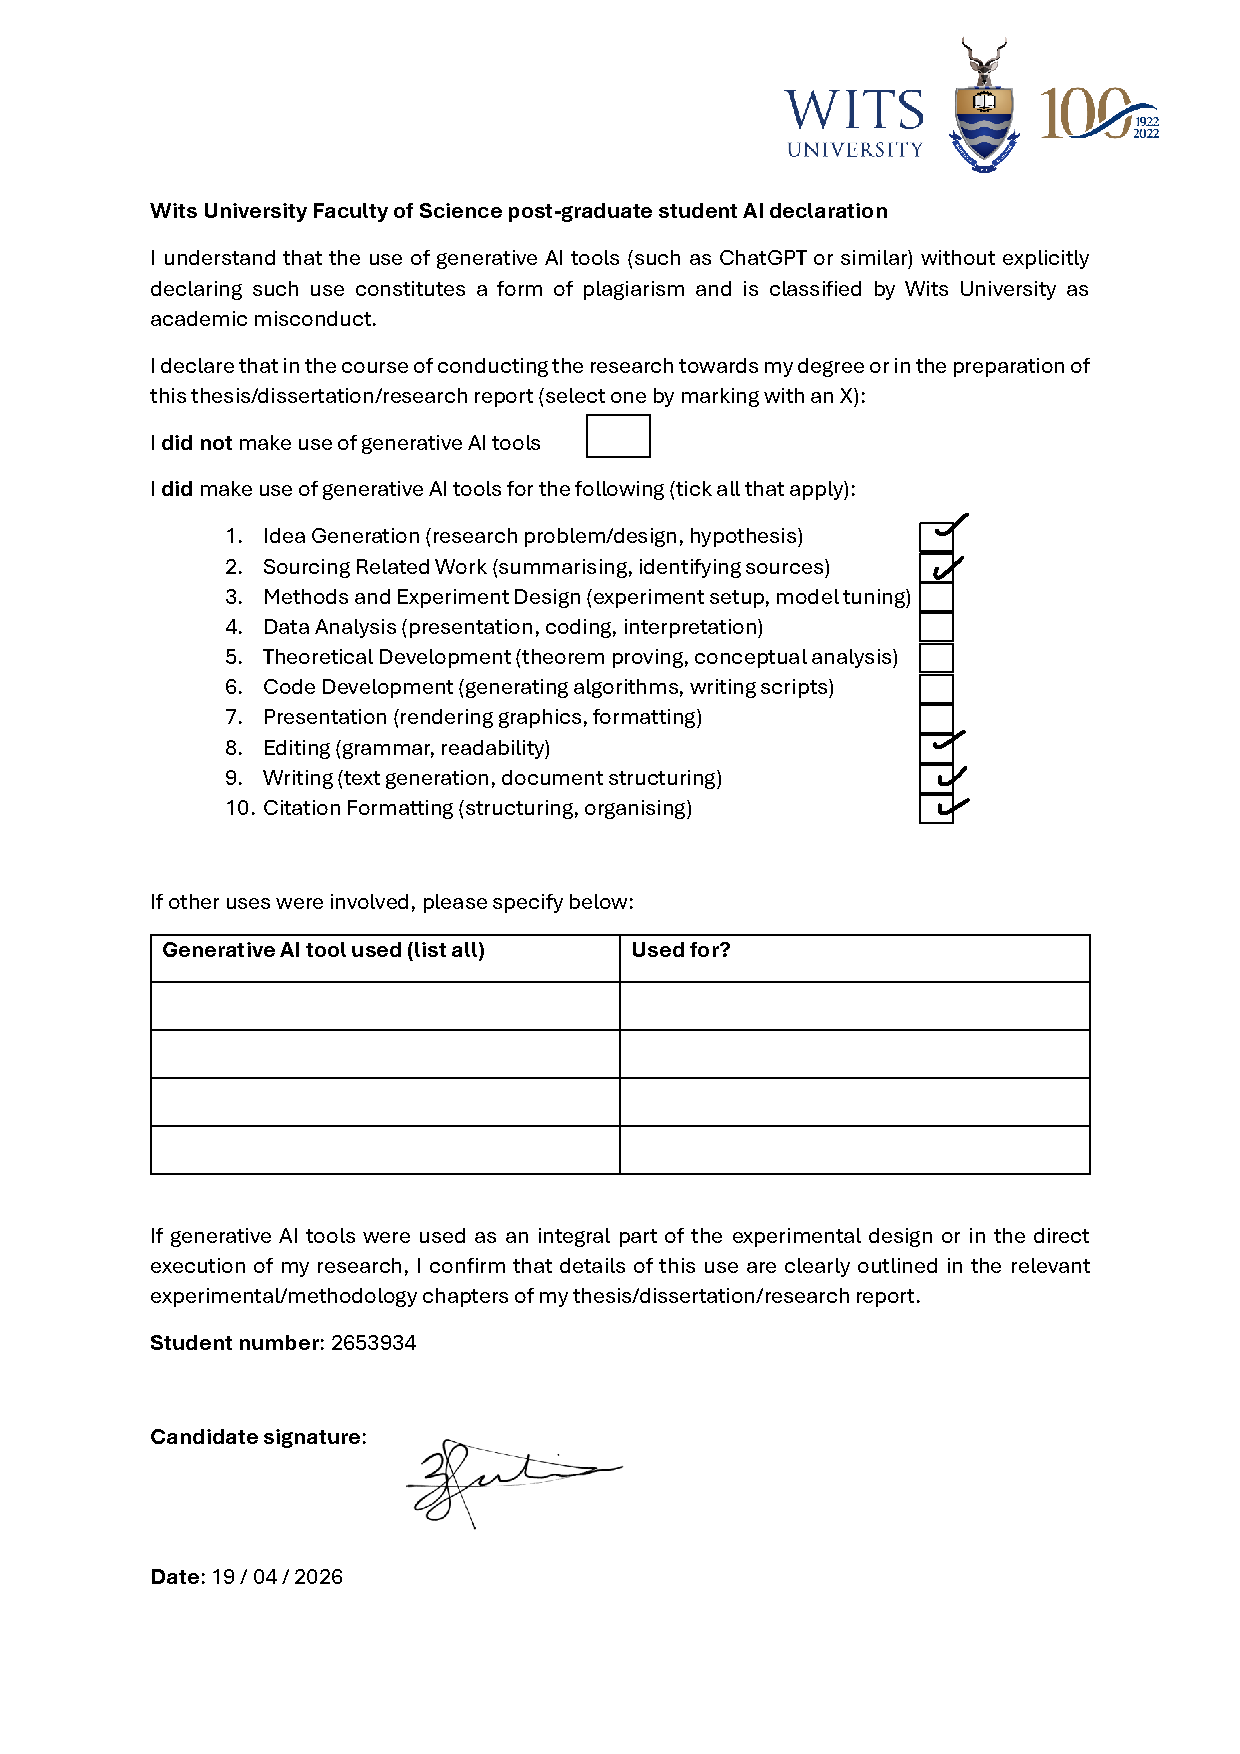
\includepdf[pages=-]{PG student AI declaration LR.pdf}
\end{document}
